%____________________________________________________________________________||
%FIXME: undefined reference to new systematic section
\section{Issues with the QCD simulation and potential solutions}
\label{app:qcdMC}

We observe a mismodelling in the QCD simulation that results in a
large number of predicted events with lead jets that have a charged
hadron energy fraction close to one. This is visible in
Fig.~\ref{fig:qcdCHF}. The application of recommended MET filters
supplied by the JetMET group mitigate the problem by a factor \~5.
This is due to the addition of a ``Bad Charged Hadron'' filter
designed to remove events with problematic reconstruction of charged
hadrons. After the application of the filters, however, there is still
a spike of events at high values of lead jet charged hadron fraction.
A veto on all events with lead jet charged hadron fraction greater
than 95\% is therefore applied on the analysis signal region and QCD
sideband. 

\begin{figure}[h!]
  \begin{center}
    \subfigure[{QCD simulation with no MET filters applied}]{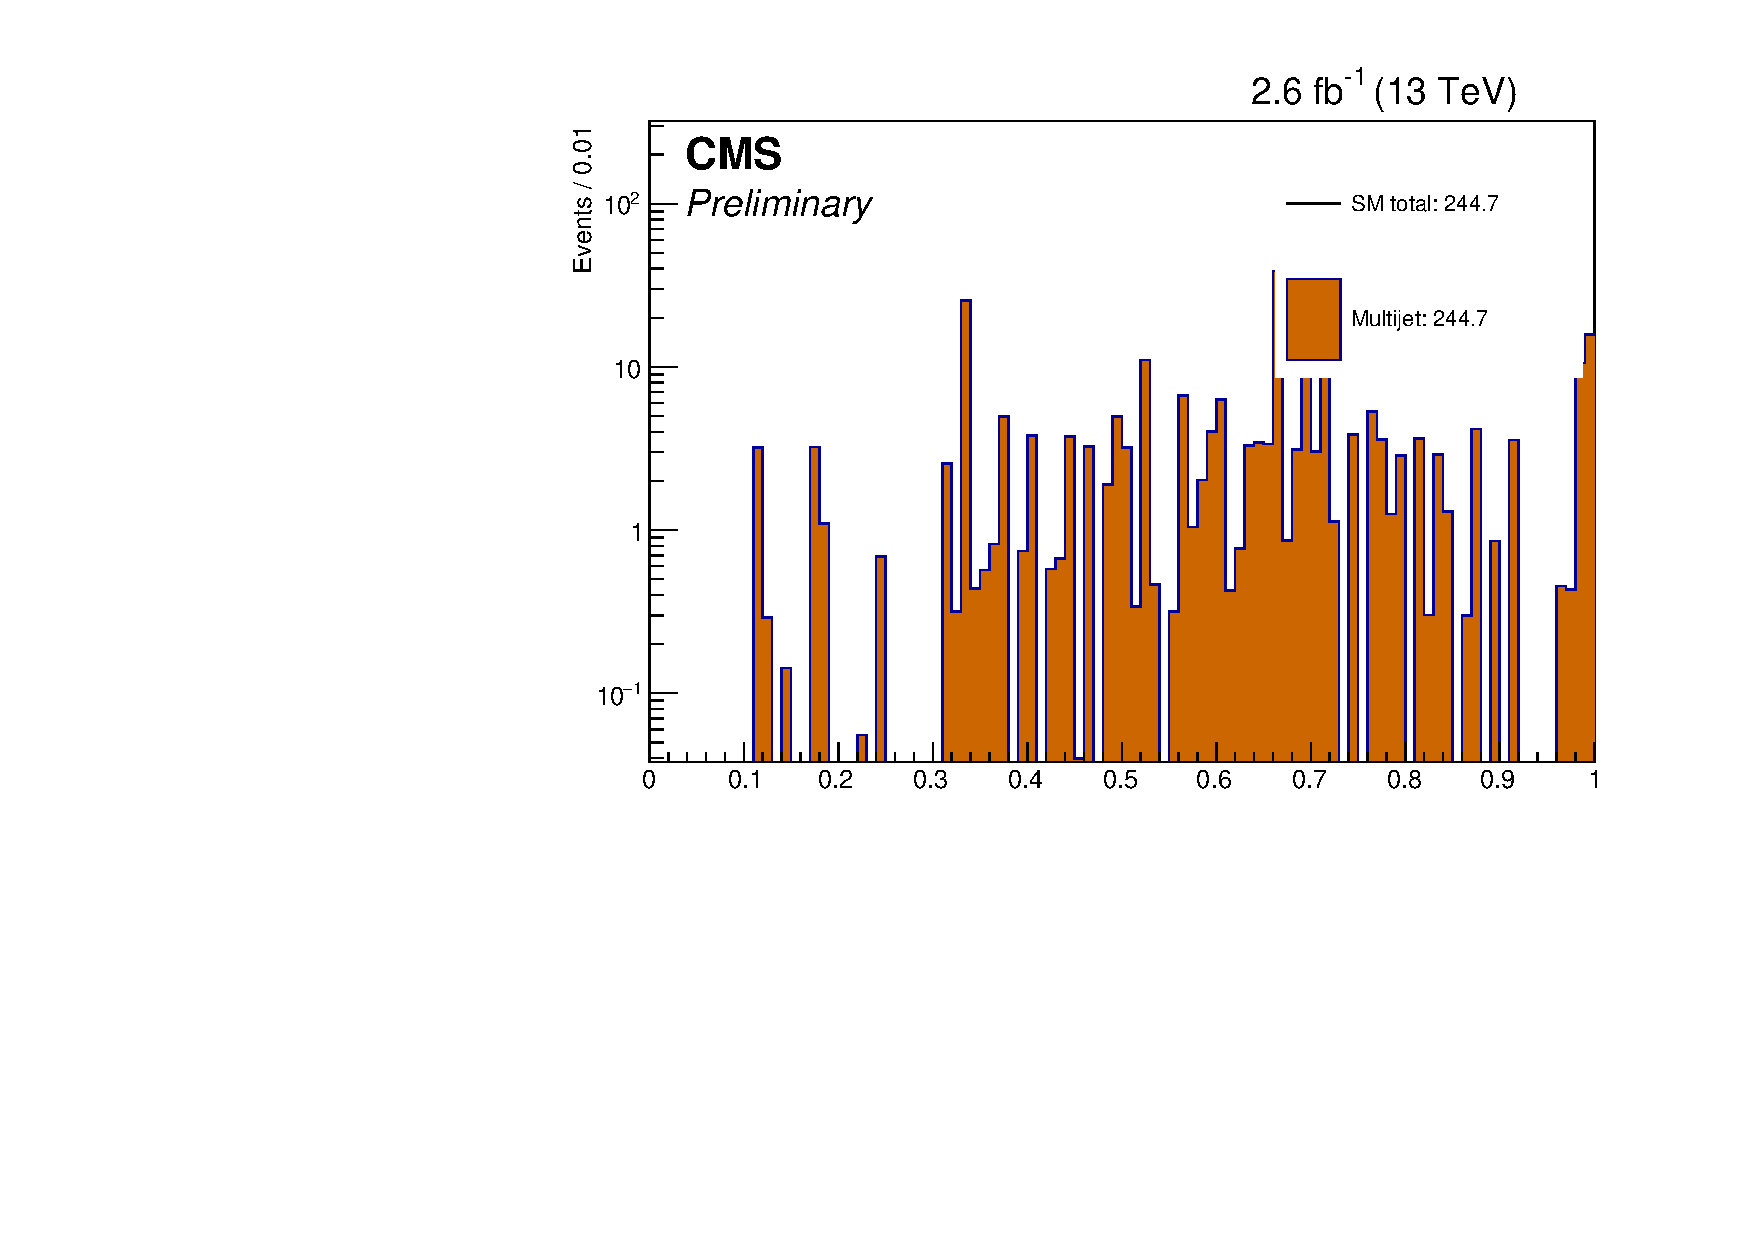
\includegraphics[width=0.5\textwidth]{figures/qcdMC/jet_chHEF_filters}} ~~
    \subfigure[{QCD simulation with MET filters applied}]{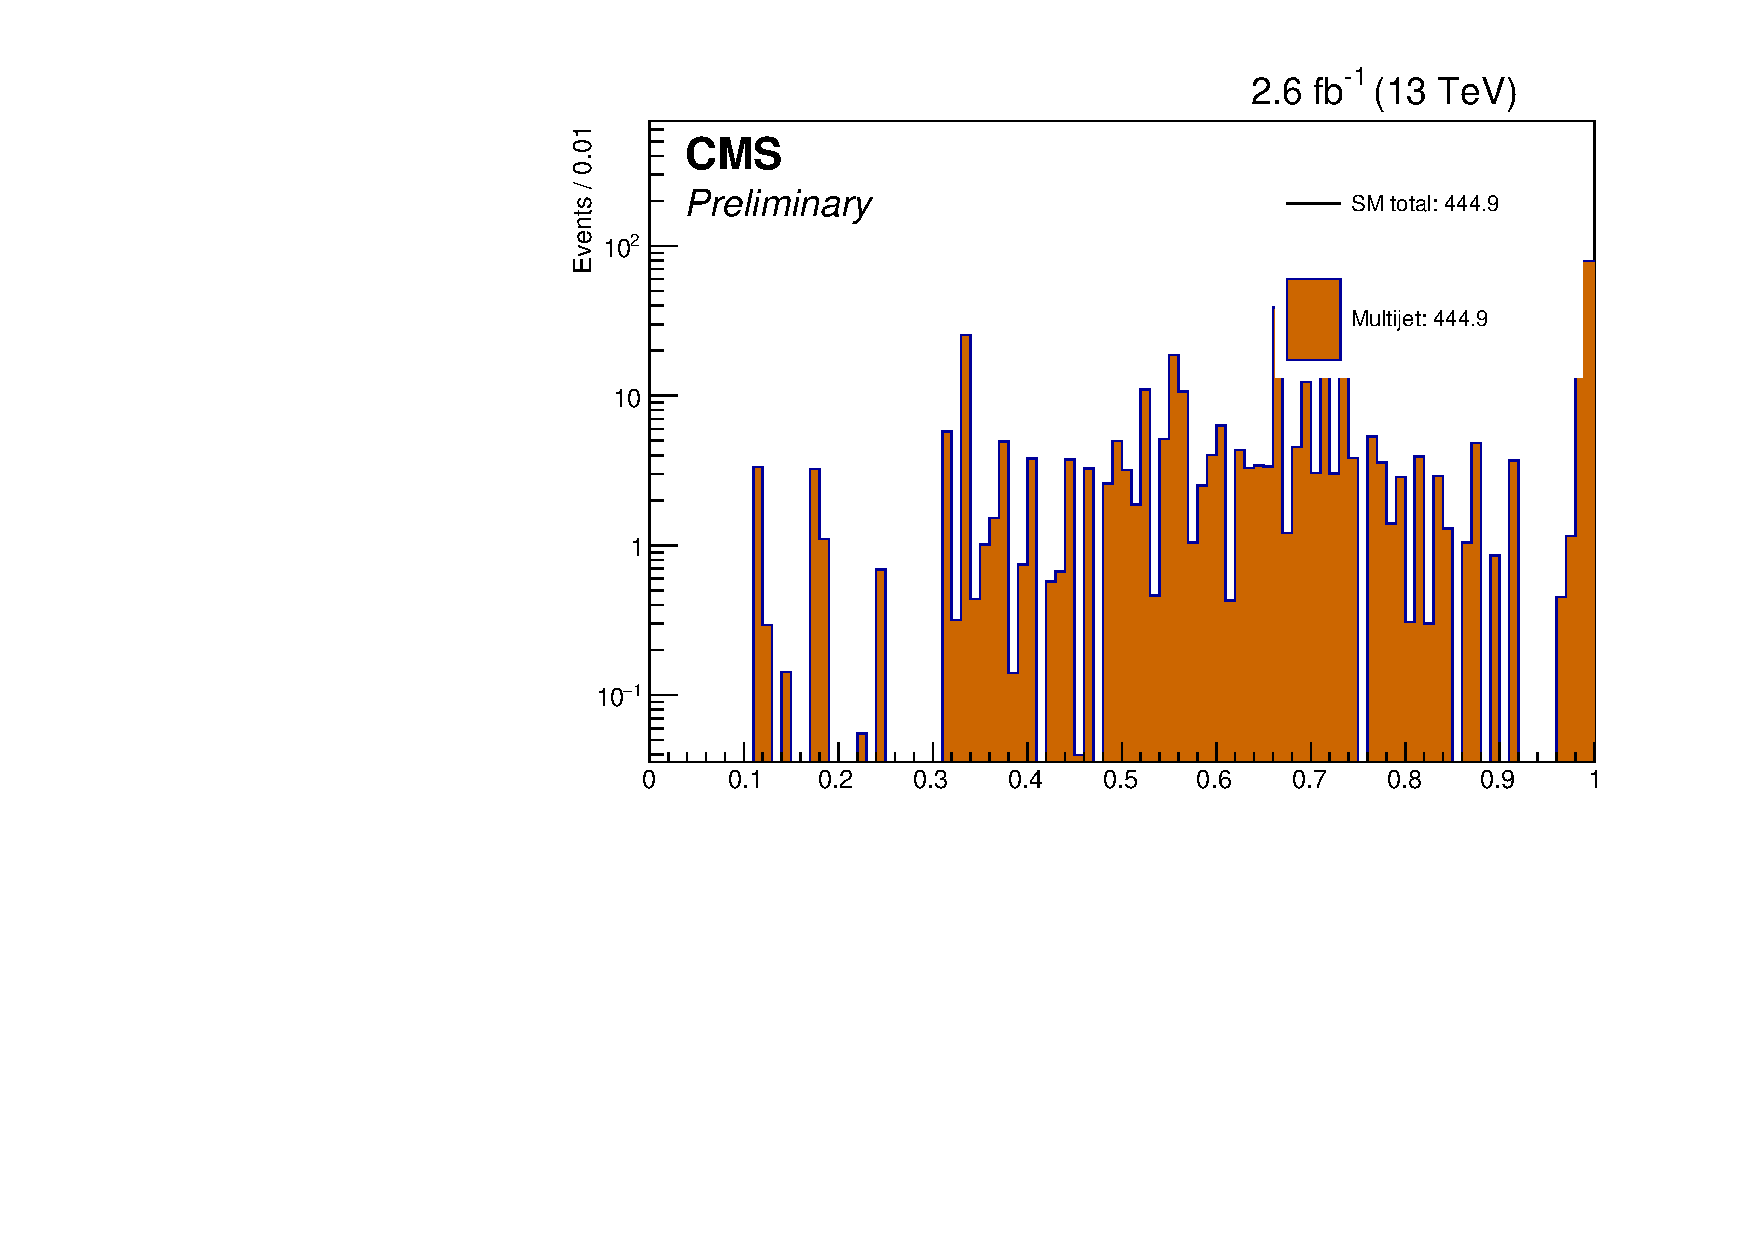
\includegraphics[width=0.5\textwidth]{figures/qcdMC/jet_chHEF_noFilters}} 
    \caption{ The lead jet charged hadron energy fraction predicted in QCD
    simulation are plotted in the case in which MET filters are
    applied and in which they aren't. A mismodelling in the QCD
    simulation causes a spike in events with lead jets that have a
    charged hadron energy fraction close to one. This this mitigated
    by the application of the MET filters.
    }
    \label{fig:qcdCHF}
  \end{center} 
\end{figure}

The dependence of the effect on pileup was also investigated. The
charged hadron energy fraction for lead jets is plotted for ``low''
pileup events with less than 16 reconstructed vertices along with
``high'' pileup events with greater than 16 reconstructed vertices.
This is shown in Fig.~\ref{fig:qcdPU}. There is no observed dependence
of the quantity on pileup.

\begin{figure}[h!]
  \begin{center}
    \subfigure[{QCD simulation with number of reconstructed vertices < 16
    }]{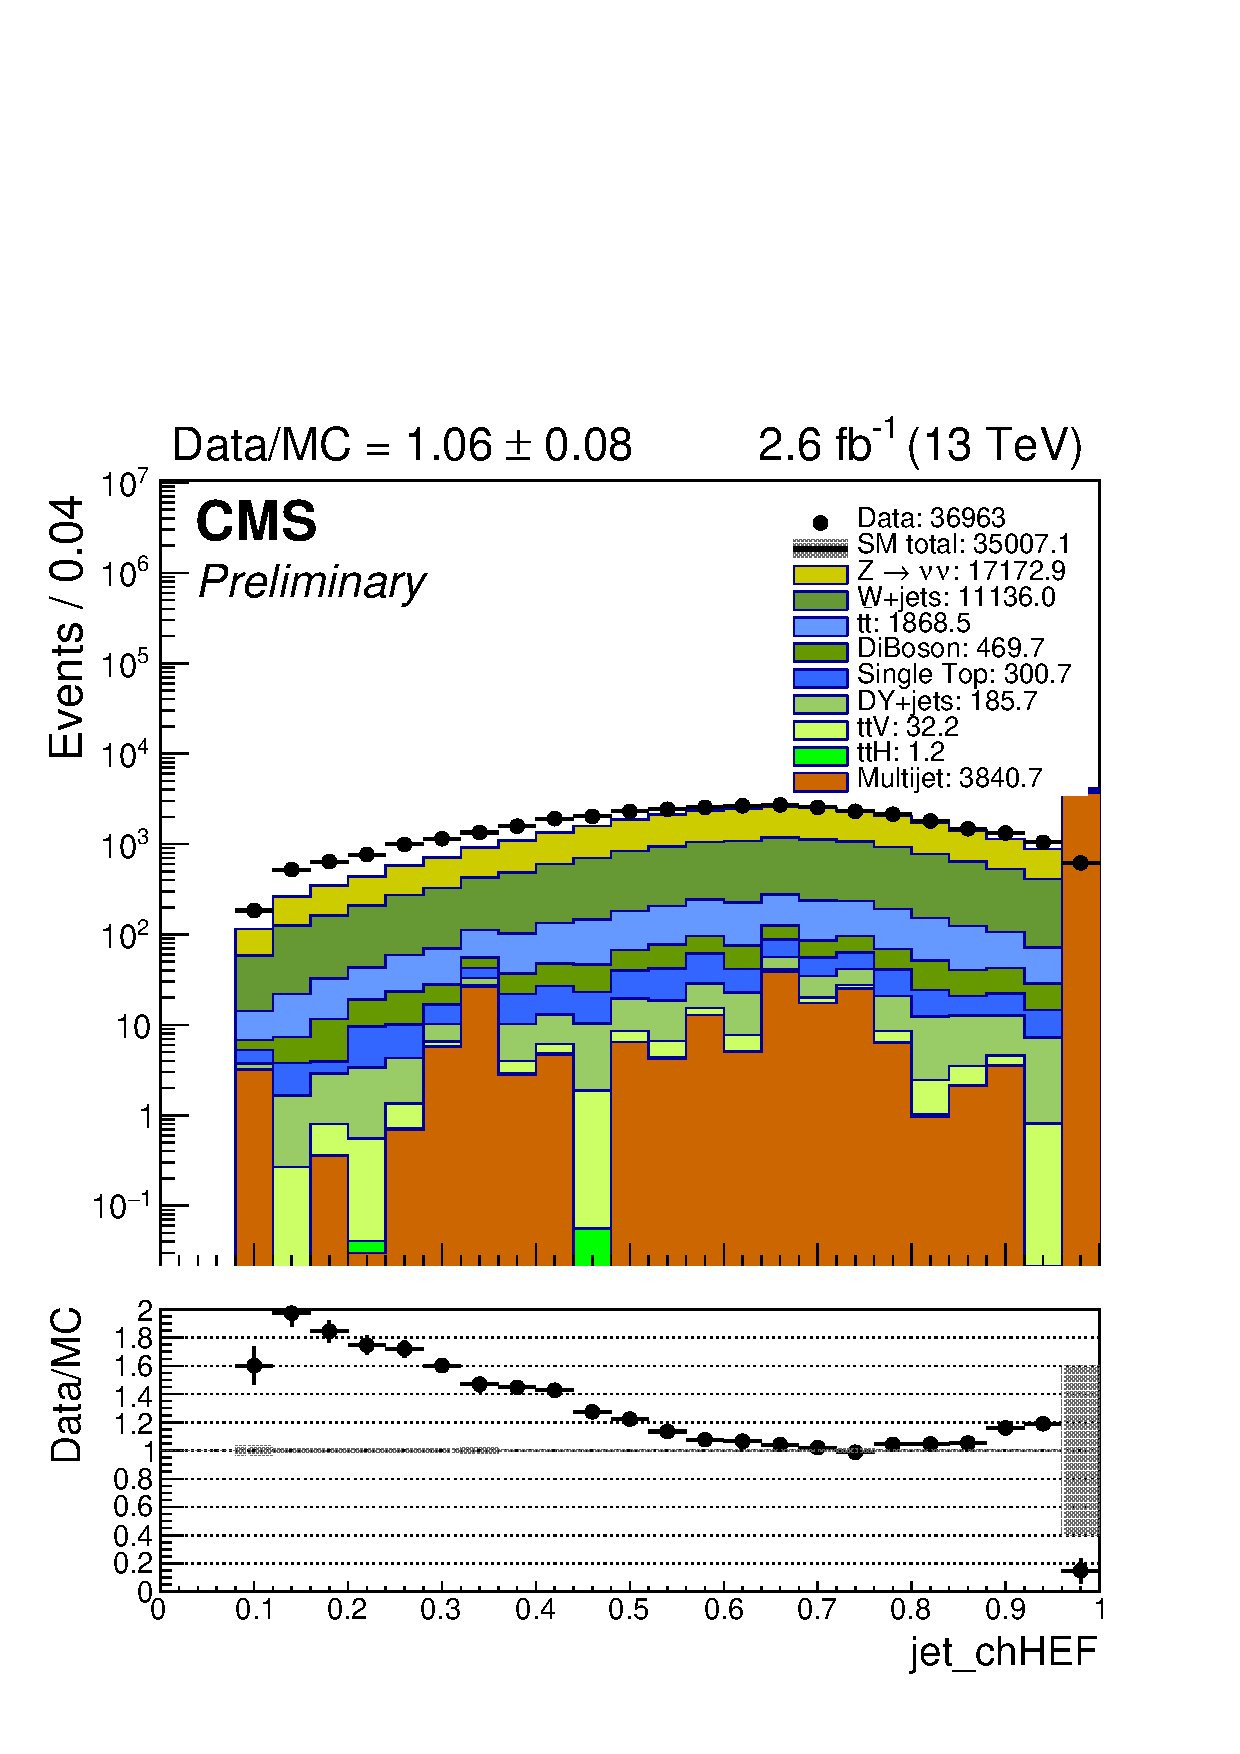
\includegraphics[width=0.5\textwidth]{figures/qcdMC/jet_chHEF_lowPU}} ~~
    \subfigure[{QCD simulation with number of reconstructed vertices >
    16
    }]{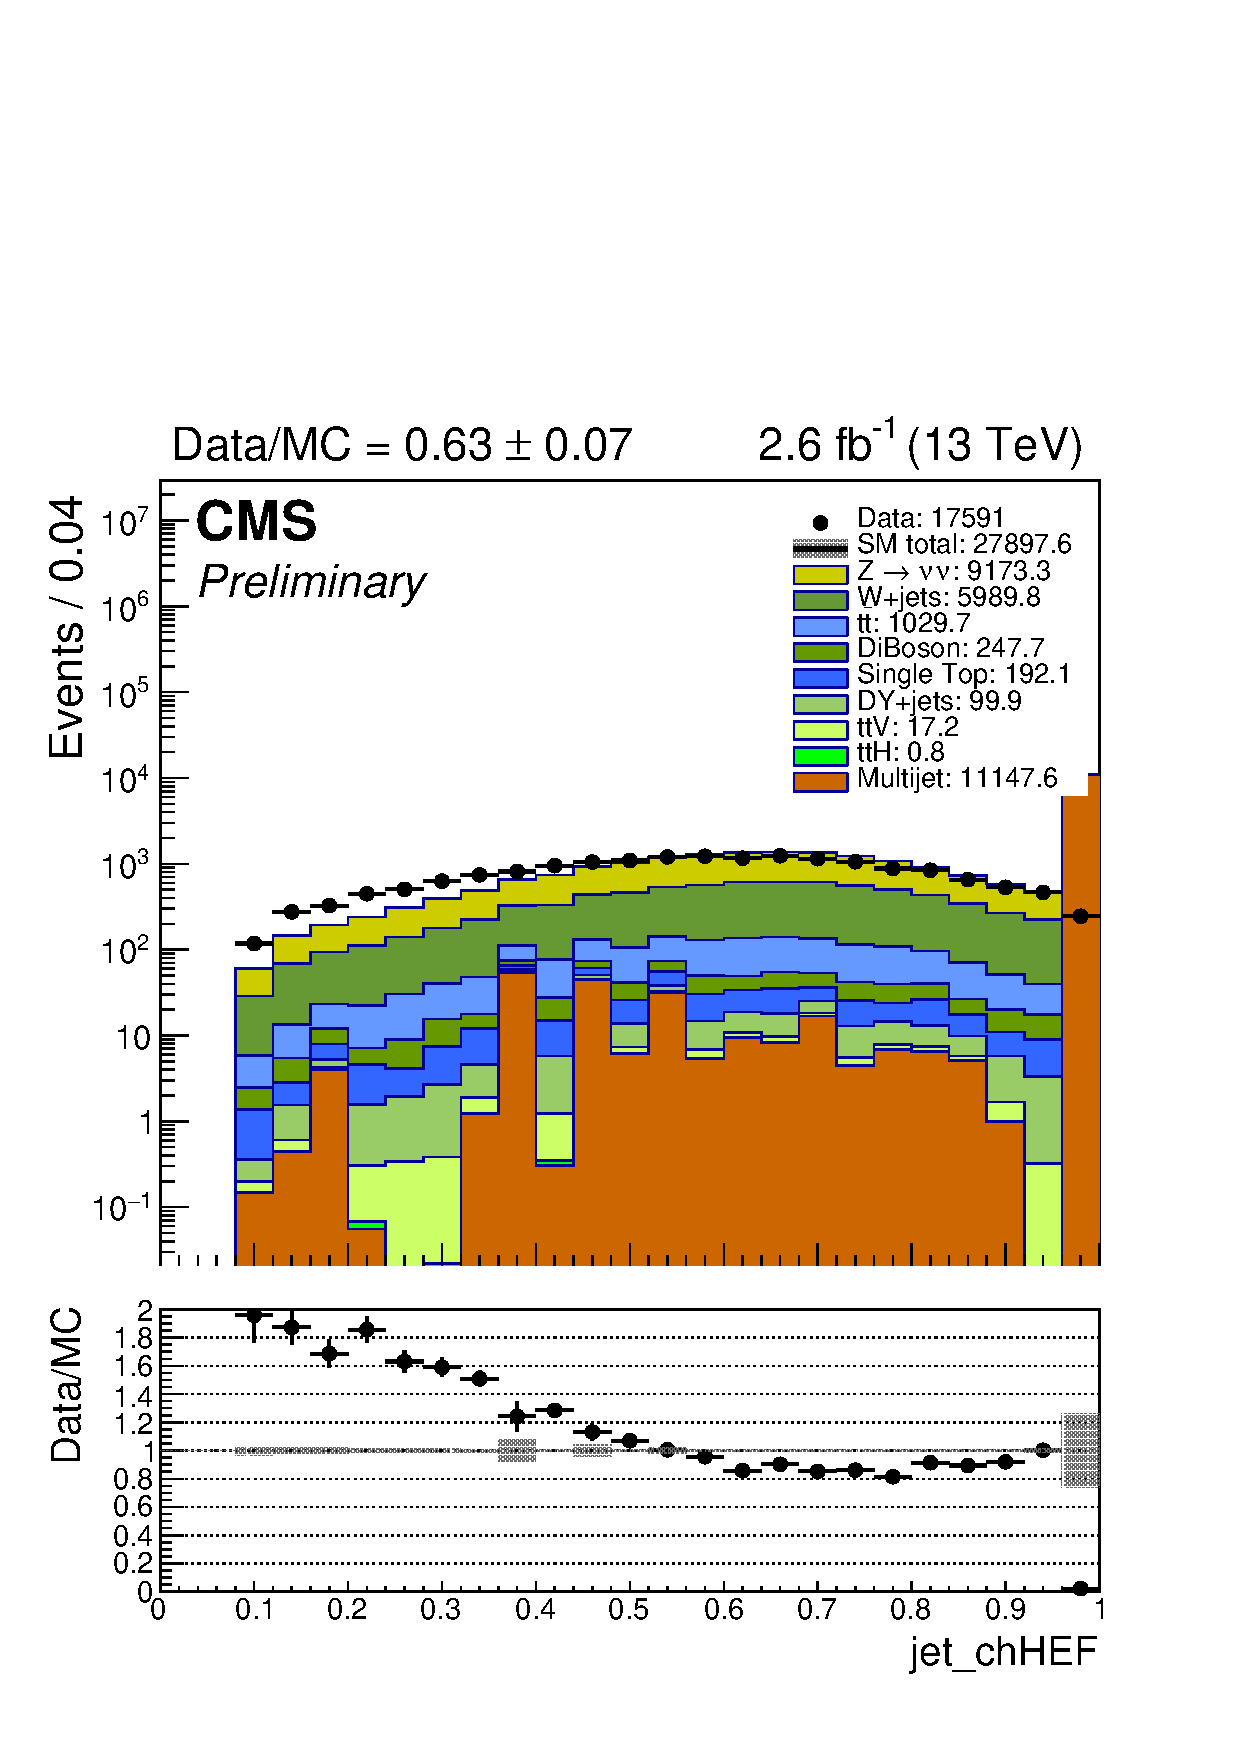
\includegraphics[width=0.5\textwidth]{figures/qcdMC/jet_chHEF_highPU}} 
    \caption{ The lead jet charged hadron energy fraction predicted in QCD
    simulation are plotted for low and high pileup.    }
    \label{fig:qcdPU}
  \end{center} 
\end{figure}
